\section{Ramp Rate Analysis} %4.5
\label{section4.5}

From Section~\ref{section3.5}, we understand how important to use ramp rate in power system. The aim is to be realistic. This is a real constraint in physical systems. The control cannot be used in reality if do not set the limit of it.

\begin{equation}
    Rate = \frac{P_{\sys{peak}} - P_o}{\sys{PeakTime}}
\end{equation}



\begin{table}[htbp]
  \centering
    \begin{tabular}{ccccc}
    Generator & Pnom (MW) & 1\% Pnom per min (MW/min) & 1\% Pnom per sec (MW/sec)\\
    g6    & 360   & 3.6   & 0.06\\
    g7    & 180   & 1.8   & 0.03\\
    g14   & 630   & 6.3   & 0.105\\
    g15   & 1080  & 10.8  & 0.18\\
    g16   & 630   & 6.3   & 0.105\\
    \end{tabular}
  \caption{Nominal ramp rate of generators}
  \label{4_5_nominal_rate}
\end{table}



\begin{table*}[htbp]
\centering
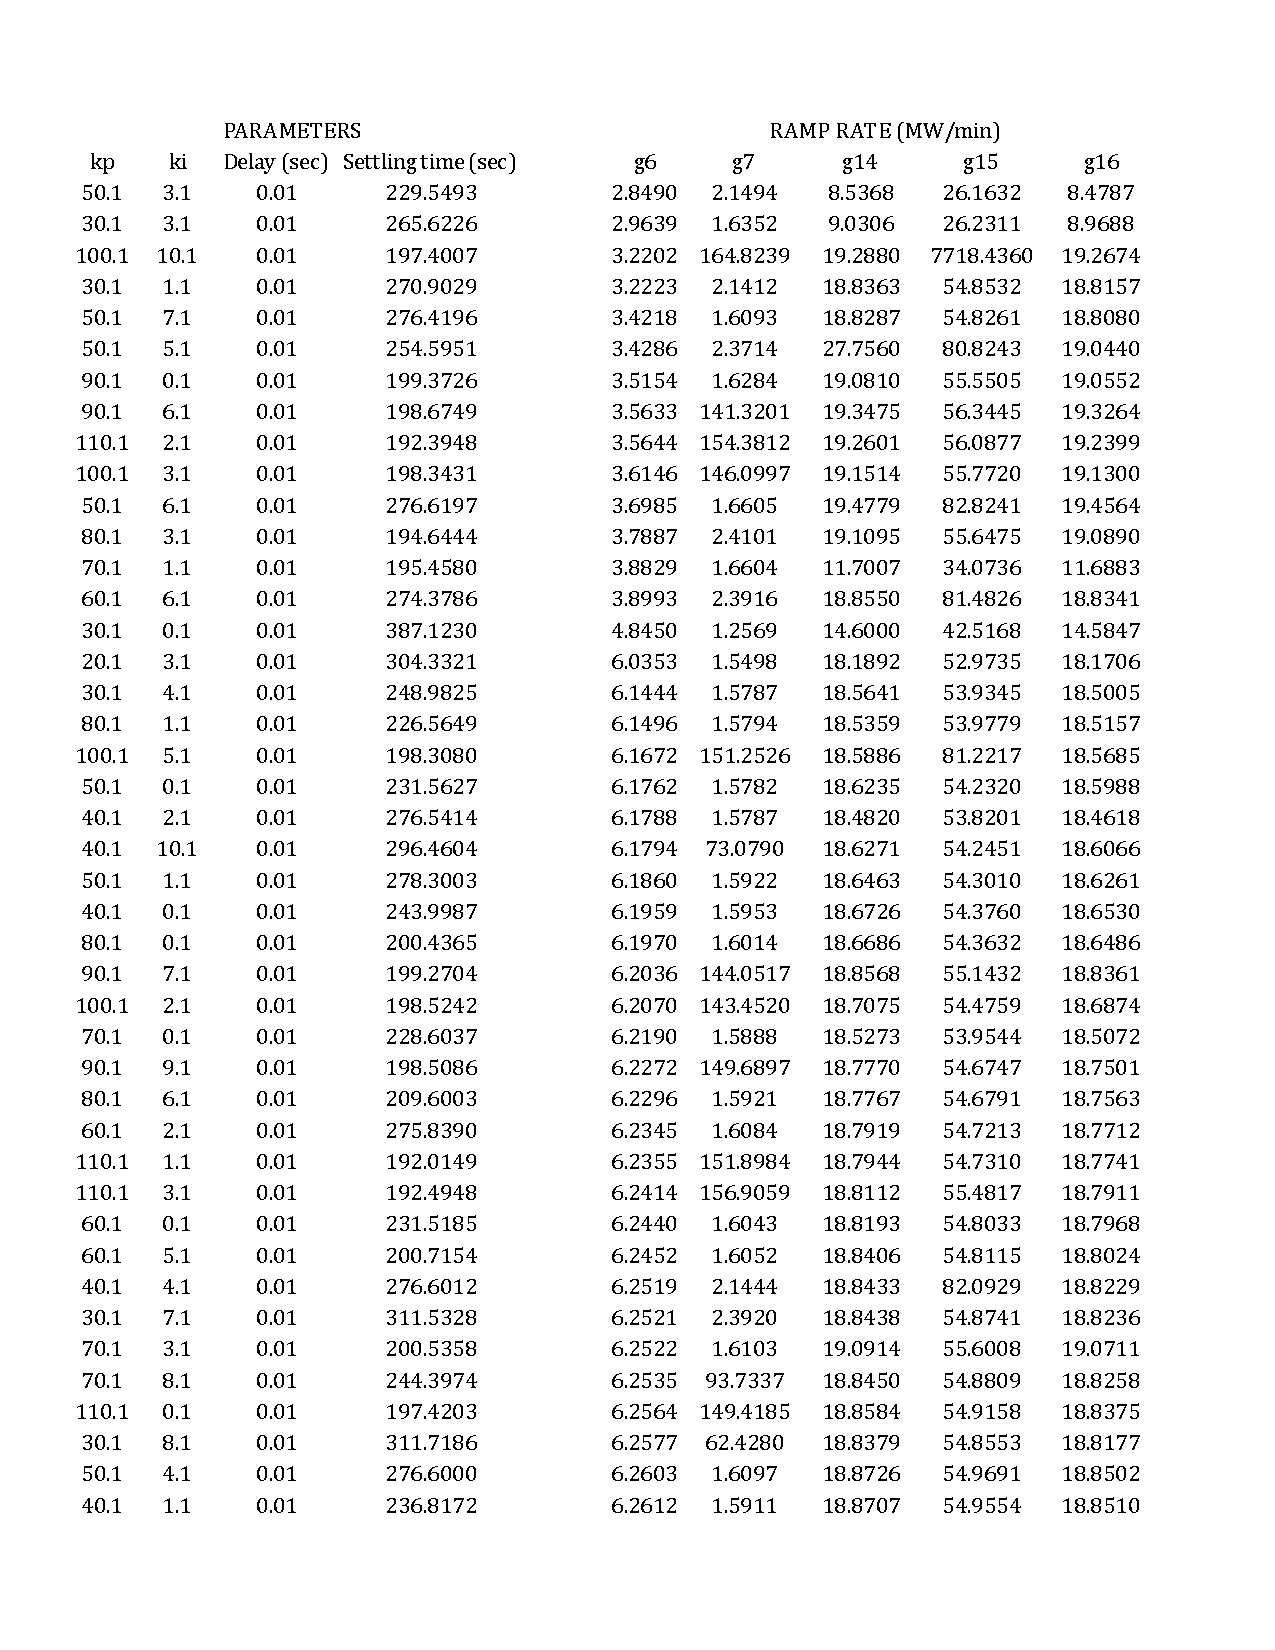
\includegraphics[width = \textwidth]{figure/4_5_risk.pdf}
\caption{Generators' real ramp rates, ranked by g6's ramp rate.}
\label{4_5_risk}
\end{table*}